\section{Messergebnisse und Auswertung}
\subsection{Variabler Auftreffpunkt \texorpdfstring{$x_0$}{x0}}
Für jede Messreihe (konstante Periodendauer $T$) werden die Differenzenfrequenzen $\Delta \nu$ aus der Anzahl der Maxima $N$ und dem zeitlichen 
Abstand $\Delta t$ berechnet.
\begin{equation}
  \label{eq:delta_nu}
  \Delta \nu = \frac{N}{\Delta t}, \qquad s_{\Delta \nu} = \Delta \nu \cdot \frac{s_{\Delta t}}{\Delta t} = \frac{N \cdot s_{\Delta t}}{\Delta t^2}
\end{equation}
Der Fehler der Zeitdifferenz $\Delta t$ wurde auf $s_{\Delta t} = 10$\,\textmu s abgeschätzt.\footnote{Dies ist das 5-fache des protokollierte Fehlers, da 
zusätzliche Fehler auftreten, die nicht von der Bestimmung des Maximums herrühren.} \\
Aus \autoref{eq:alpha:exp} folgt:
\begin{equation}
  \label{eq:x0:m}
  x_0(\Delta \nu) = \frac{\lambda \cdot L}{2 \cdot n \cdot d \cdot \omega \cdot \alpha} \cdot \Delta \nu =: m \cdot \Delta \nu
\end{equation}
Allerdings unterscheidet sich der gemessene Auftreffpunkt $x_0'$ aufgrund des Messaufbaus um einem Skalenoffset $x_m$, 
welcher noch berücksichtigt werden muss.
\begin{equation}
  x_0' = x_0 - x_m
\end{equation}
Die Daten können also mit folgender Formel beschrieben werden:
\begin{equation}
  x_0(\Delta \nu) = m \cdot \Delta \nu + x_m
\end{equation}
Die gemessenen Werte werden nun in ein $x_0'$ - $\Delta \nu$ -Diagramm eingetragen und mit der obigen Formel gefittet 
(\autoref{img:fit:x0:30ms}, \autoref{img:fit:x0:45ms} und \autoref{img:fit:x0:60ms}). Durch diese Wahl der Koordinatenachsen kann der Offset $x_m$ 
nun direkt abgelesen werden.
Der geschätzte Fehler auf $x_0'$ beträgt $s_{x_0'} = 0.05$\,mm. Die Ergebnisse sind in \autoref{tab:fit:x0} dargestellt.

\begin{figure}[H]
\begin{center}
  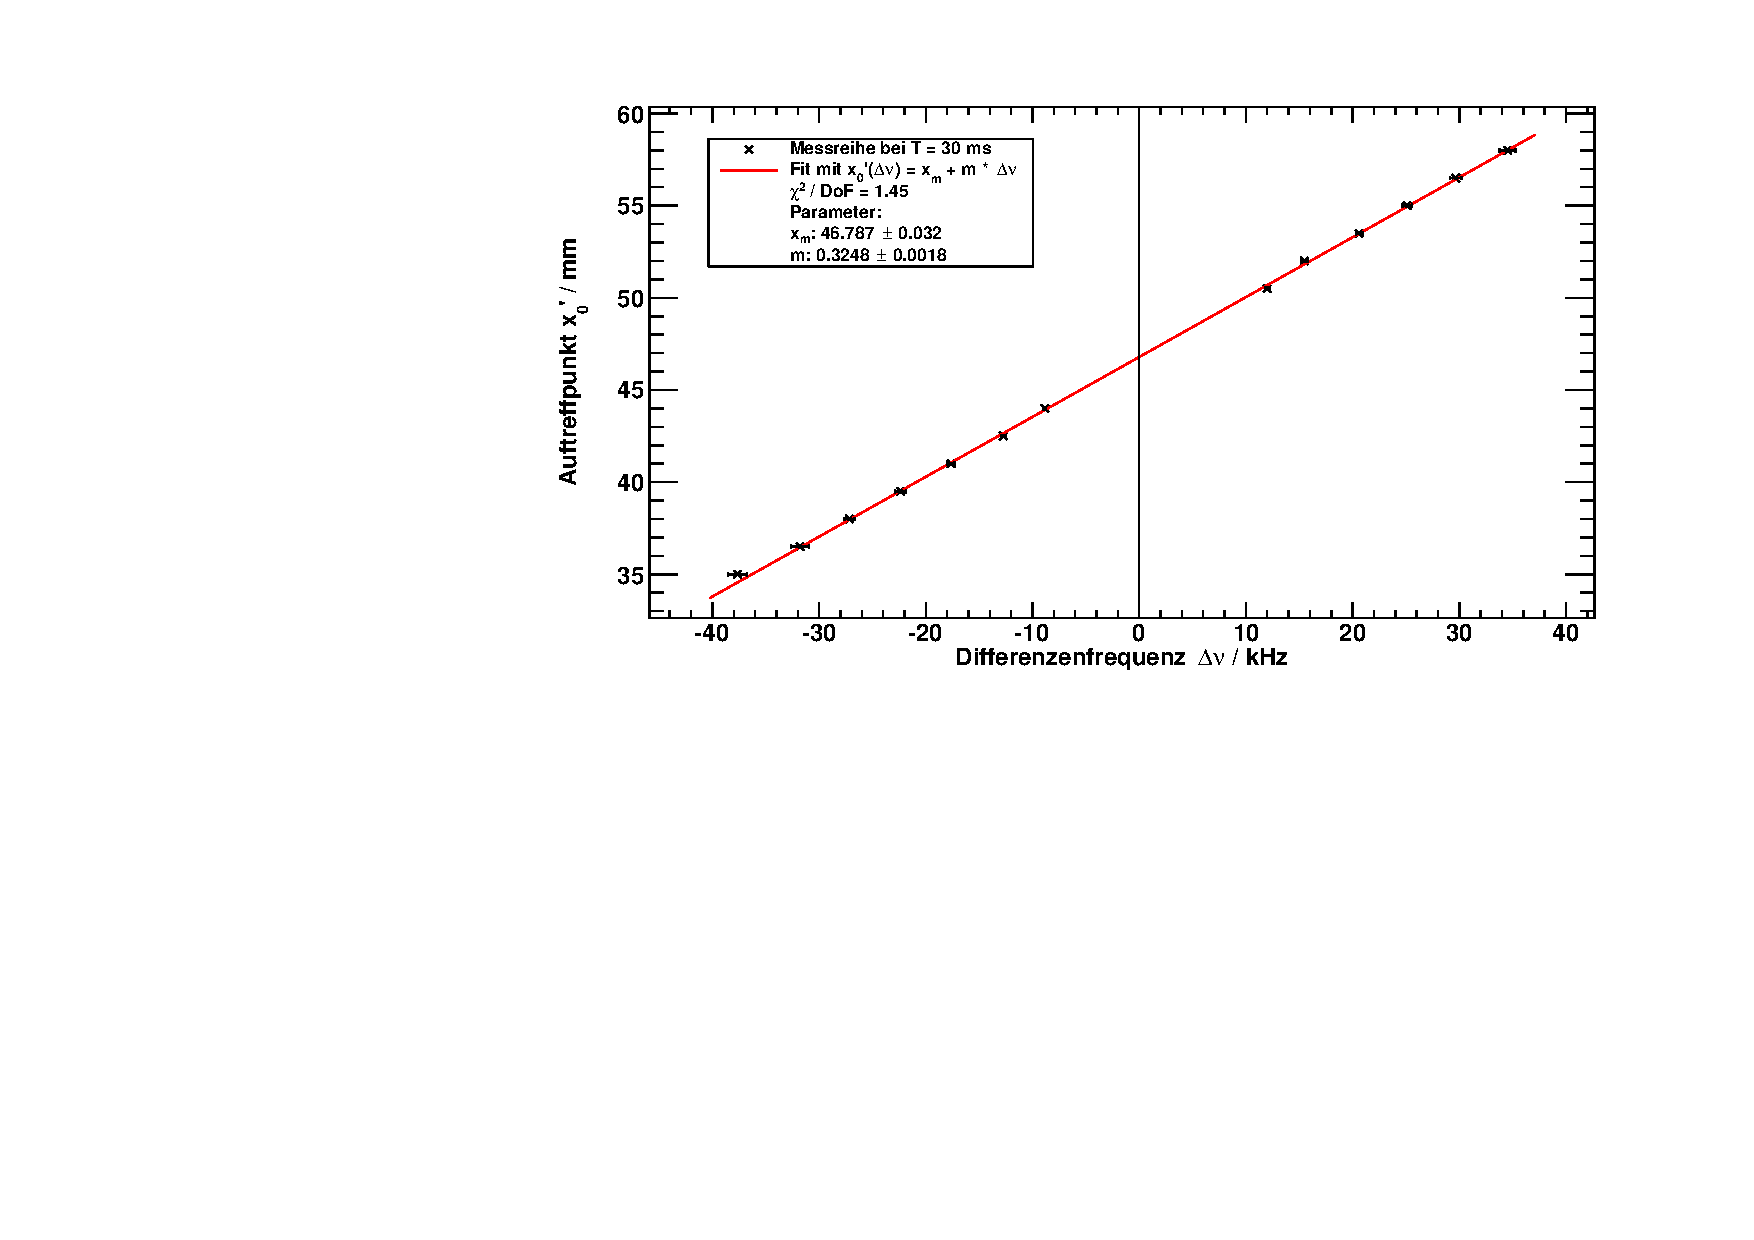
\includegraphics[width=\textwidth]{../img/fit_T_30ms.pdf}
  \caption{Linearer Fit von $x_0'$ bei $T = 30$\,ms.}.
  \label{img:fit:x0:30ms}
\end{center}
\end{figure}

\begin{figure}[H]
\begin{center}
  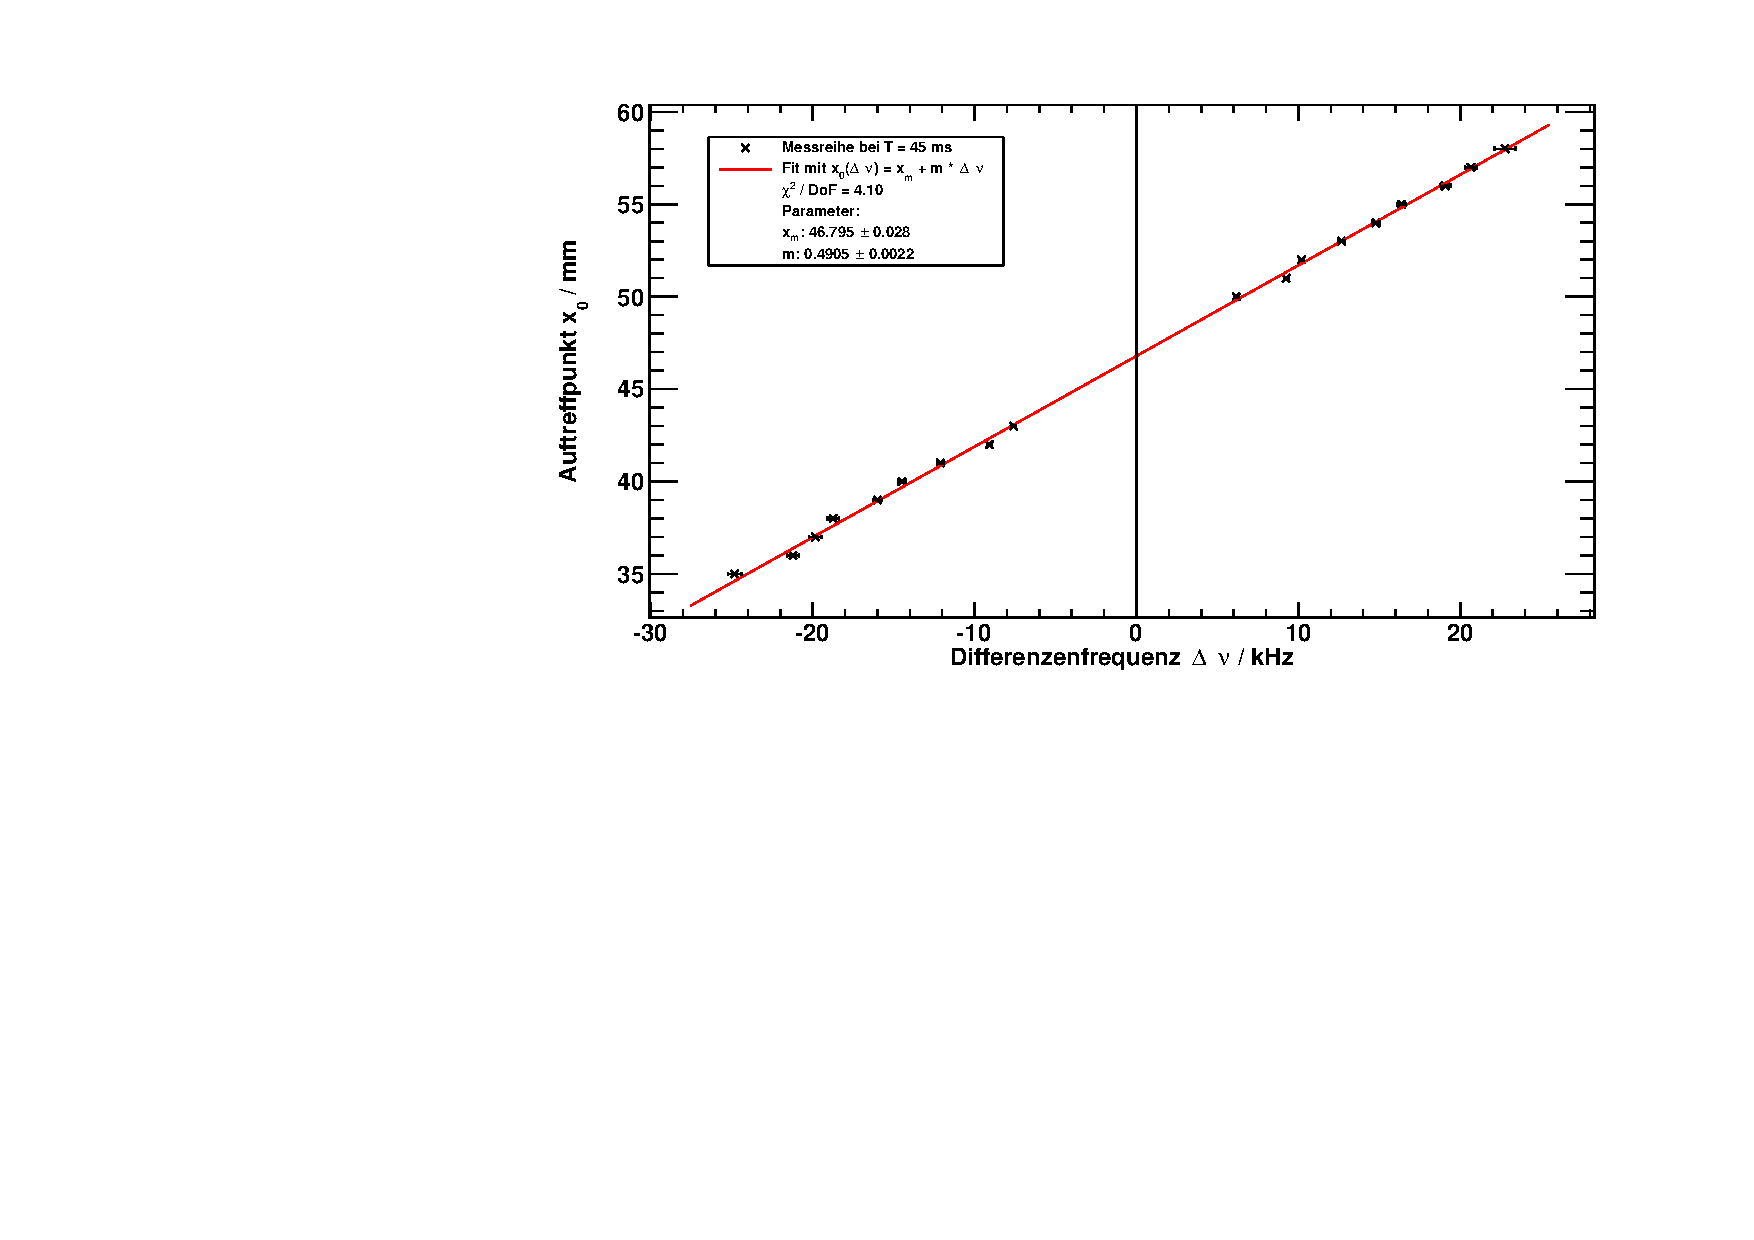
\includegraphics[width=\textwidth]{../img/fit_T_45ms.pdf}
  \caption{Linearer Fit von $x_0'$ bei $T = 45$\,ms.}.
  \label{img:fit:x0:45ms}
\end{center}
\end{figure}

\begin{figure}[H]
\begin{center}
  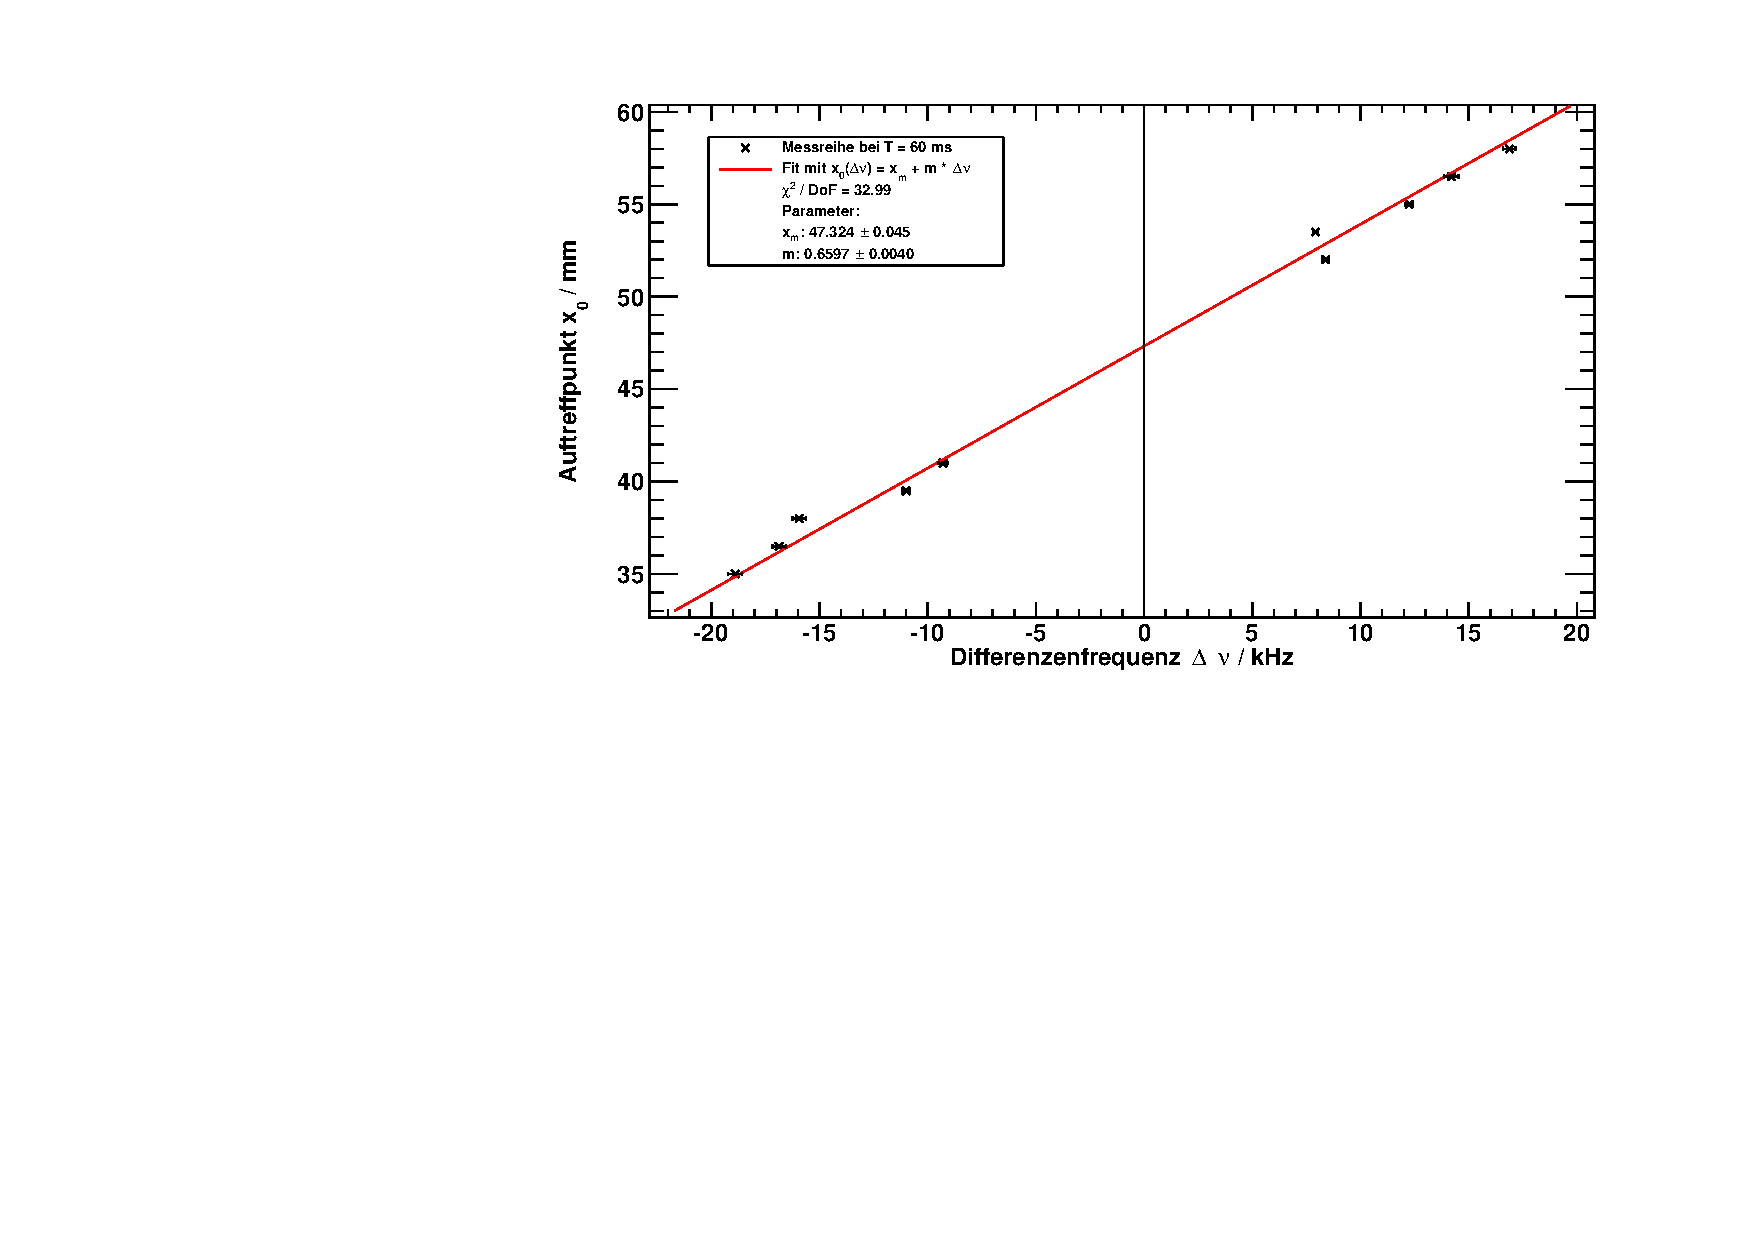
\includegraphics[width=\textwidth]{../img/fit_T_60ms.pdf}
  \caption{Linearer Fit von $x_0'$ bei $T = 60$\,ms.}.
  \label{img:fit:x0:60ms}
\end{center}
\end{figure}

\begin{table}[H]
\caption{Fitergebnisse von $x_0'(\Delta \nu)$ bei festen Periodendauern $T$.}
\begin{center}
\begin{tabular}{|c|c|c|c|c|}
  \hline
  $T$ / ms & $x_m$ / mm & $s_{x_m}$ / mm & $m$ / (mm / kHz) & $s_m$ / (mm / kHz) \\ \hline
  30 & 46.787 & 0.032 & 0.3248 & 0.0018 \\ \hline
  45 & 46.795 & 0.028 & 0.4905 & 0.0022 \\ \hline
  60 & 47.324 & 0.045 & 0.6597 & 0.0040 \\ \hline
\end{tabular}
\end{center}
\label{tab:fit:x0}
\end{table}


Der gewichtete Mittelwert aus den Offsets $x_m$ für verschiedene Periodendauern $T$ liefert:
\begin{equation}
  \label{eq:xm}
  \bar{x}_{m} = (46.886 \pm 0.019)\,\text{mm}
\end{equation}
Aus den einzelnen Steigungen $m$ lässt sich nun der Mitführungskoeffizient $\alpha$ nach \autoref{eq:x0:m} bestimmen. Die Werte der Konstanten des 
Versuchaufbaus sind in \autoref{sec:aufbau} aufgelistet.
\begin{equation}
  \alpha = \frac{\lambda \cdot L}{2 \cdot n \cdot d} \cdot \frac{1}{\omega \cdot m}, \qquad
  s_{\alpha} = \alpha \cdot \sqrt{\left(\frac{s_m}{m}\right)^2 + \left(\frac{s_\omega}{\omega}\right)^2}
\end{equation}
Die Kreisfrequenz $\omega$ lässt sich aus der Periodendauer folgendermaßen bestimmen:
\begin{equation}
  \label{eq:omega}
  \omega = \frac{2 \pi}{T}, \qquad s_{\omega} = \omega \cdot \frac{s_T}{T}
\end{equation}
Die berechneten Mitführungskoeffizienten sind in \autoref{tab:x0:alpha} aufgelistet.
\begin{table}[H]
\caption{Mitf\"uhrungskoeffizienten bei festen Perioden $T$. }
\begin{center}
\begin{tabular}{|c|c|c|}
  \hline
  $T$ / ms & $\alpha$ & $s_{\alpha}$ \\ \hline
  30 & 0.540 & 0.005 \\ \hline
  45 & 0.537 & 0.003 \\ \hline
  60 & 0.532 & 0.004 \\ \hline
\end{tabular}
\end{center}
\label{tab:x0:alpha}
\end{table}

Da alle Mitführungskoeffizienten innerhalb einer Standardabweichung übereinstimmen, kann der gewichtete Mittelwert $\bar{\alpha}$ gebildet werden.
\begin{equation}
  \label{eq:x0:alpha:avg}
  \bar{\alpha} = 0.536 \pm 0.002
\end{equation}

\subsection{Variabler Periodendauer \texorpdfstring{$T$}{T}}
Es werden wieder die einzelnen Differenzenfrequenzen mit \autoref{eq:delta_nu} berechnet. Hier ist der Fehler $s_{\Delta t}$ 
auf die Zeitdifferenz $\Delta t$ entweder 5 oder 10 \textmu s, je nach verwendeter Auflösung des Oszilloskops. \\
Die gemessenen Werte werden in einem $\Delta \nu$-$\omega$-Diagramm dargestellt. 
Dazu werden die einstellten Periodendauern $T$ mit \autoref{eq:omega} in Kreisfrequenzen $\omega$ umgerechnet. \\
Die Daten können wieder mit einer Geraden beschrieben werden:
\begin{equation}
  \label{eq:nu_omega}
  \Delta \nu (\omega) = a + \frac{2 \cdot n \cdot d \cdot x_0 \cdot \alpha}{\lambda \cdot L} \cdot \omega  =: a + b \cdot \omega
\end{equation}
Der Offset $a$ sollte im Idealfall verschwinden, ist er jedoch nicht 0, so gibt er Information über eventuelle systematischen Fehler.
Die Fits für die verschiedenen, festen Auftreffpunkte $x_0$ sind in \autoref{img:fit:T:36mm}, \autoref{img:fit:T:40mm}, \autoref{img:fit:T:53mm} 
und \autoref{img:fit:T:57mm} dargestellt. Die Ergebnisse für den Offset $a$ und die Steigung $b$ sind in \autoref{tab:fit:T} aufgelistet.

\begin{figure}[H]
\begin{center}
  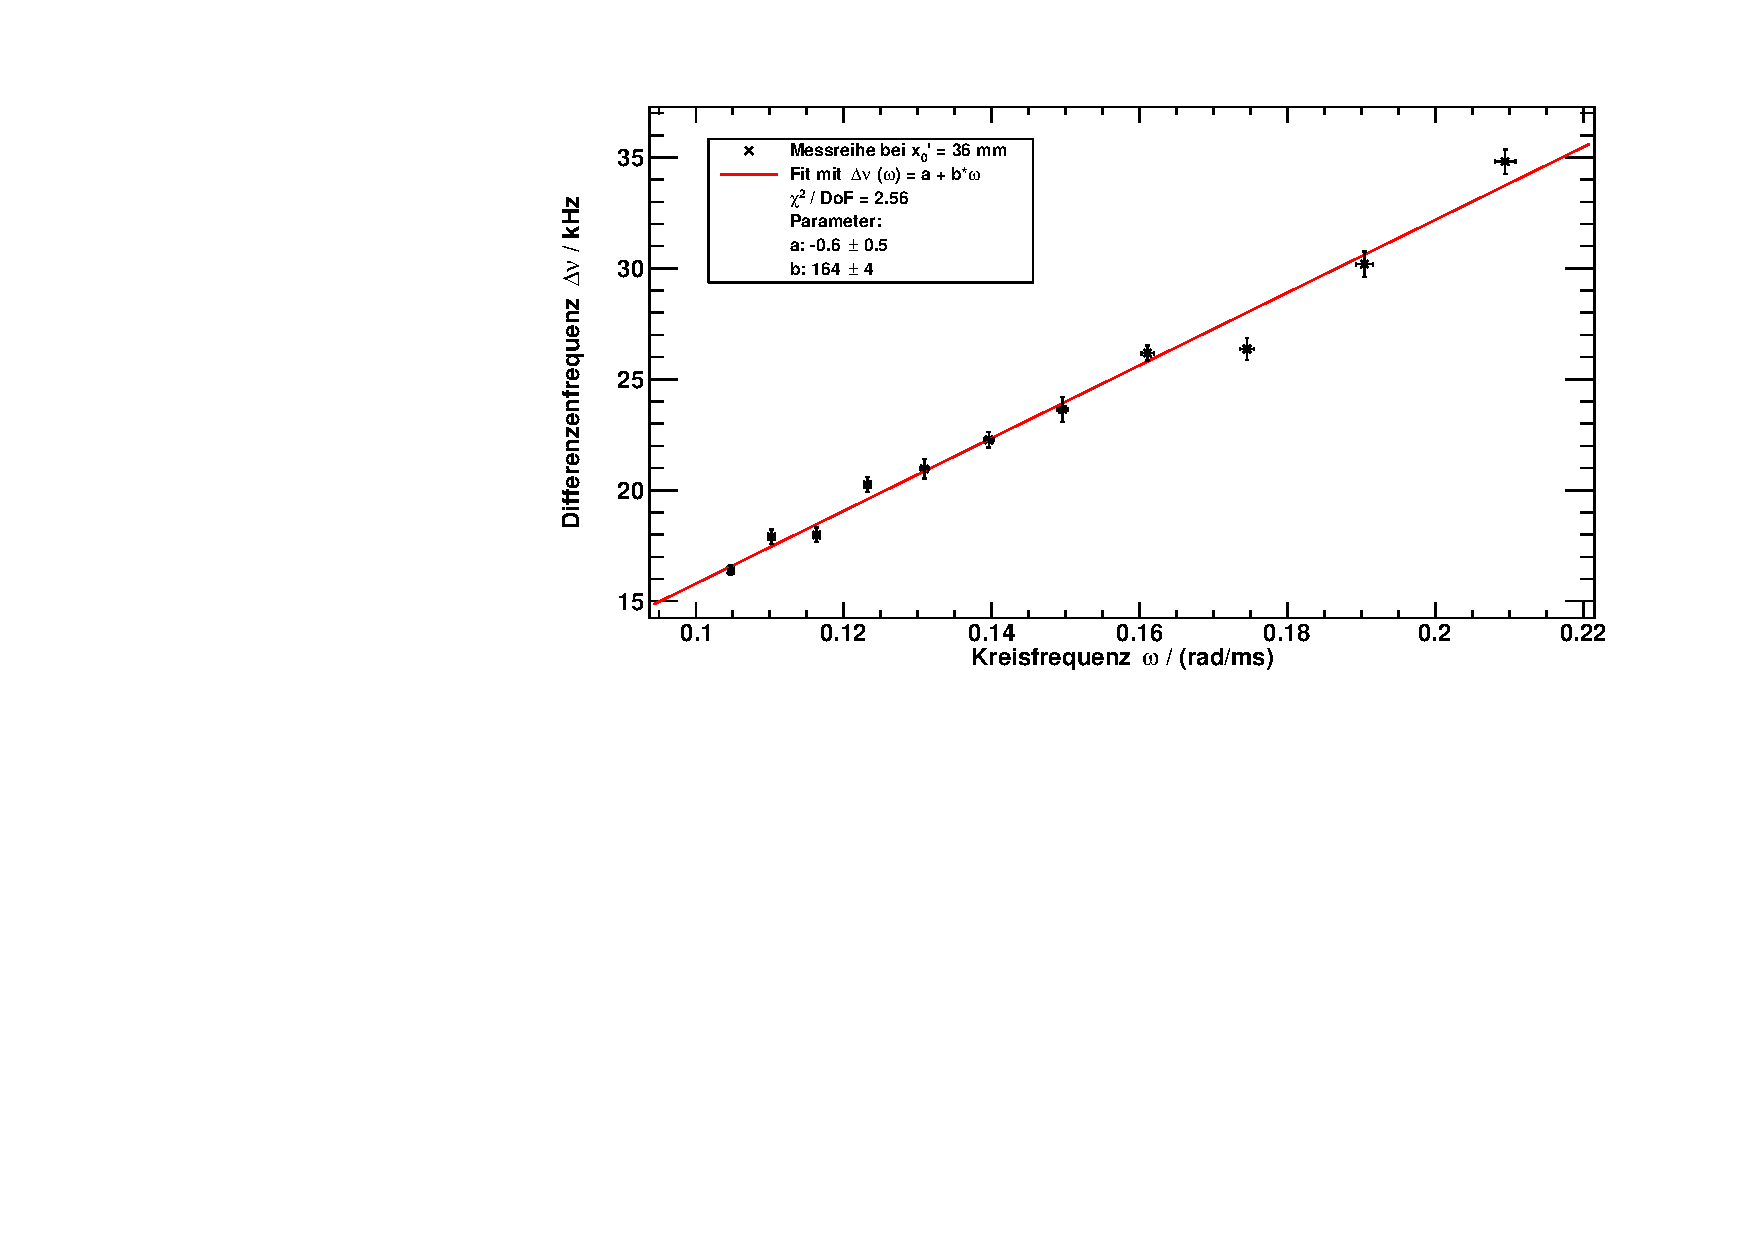
\includegraphics[width=\textwidth]{../img/fit_x0_36mm.pdf}
  \caption{Linearer Fit von $\Delta \nu$ bei $x_0' = 36$\,mm.}
  \label{img:fit:T:36mm}
\end{center}
\end{figure}

\begin{figure}[H]
\begin{center}
  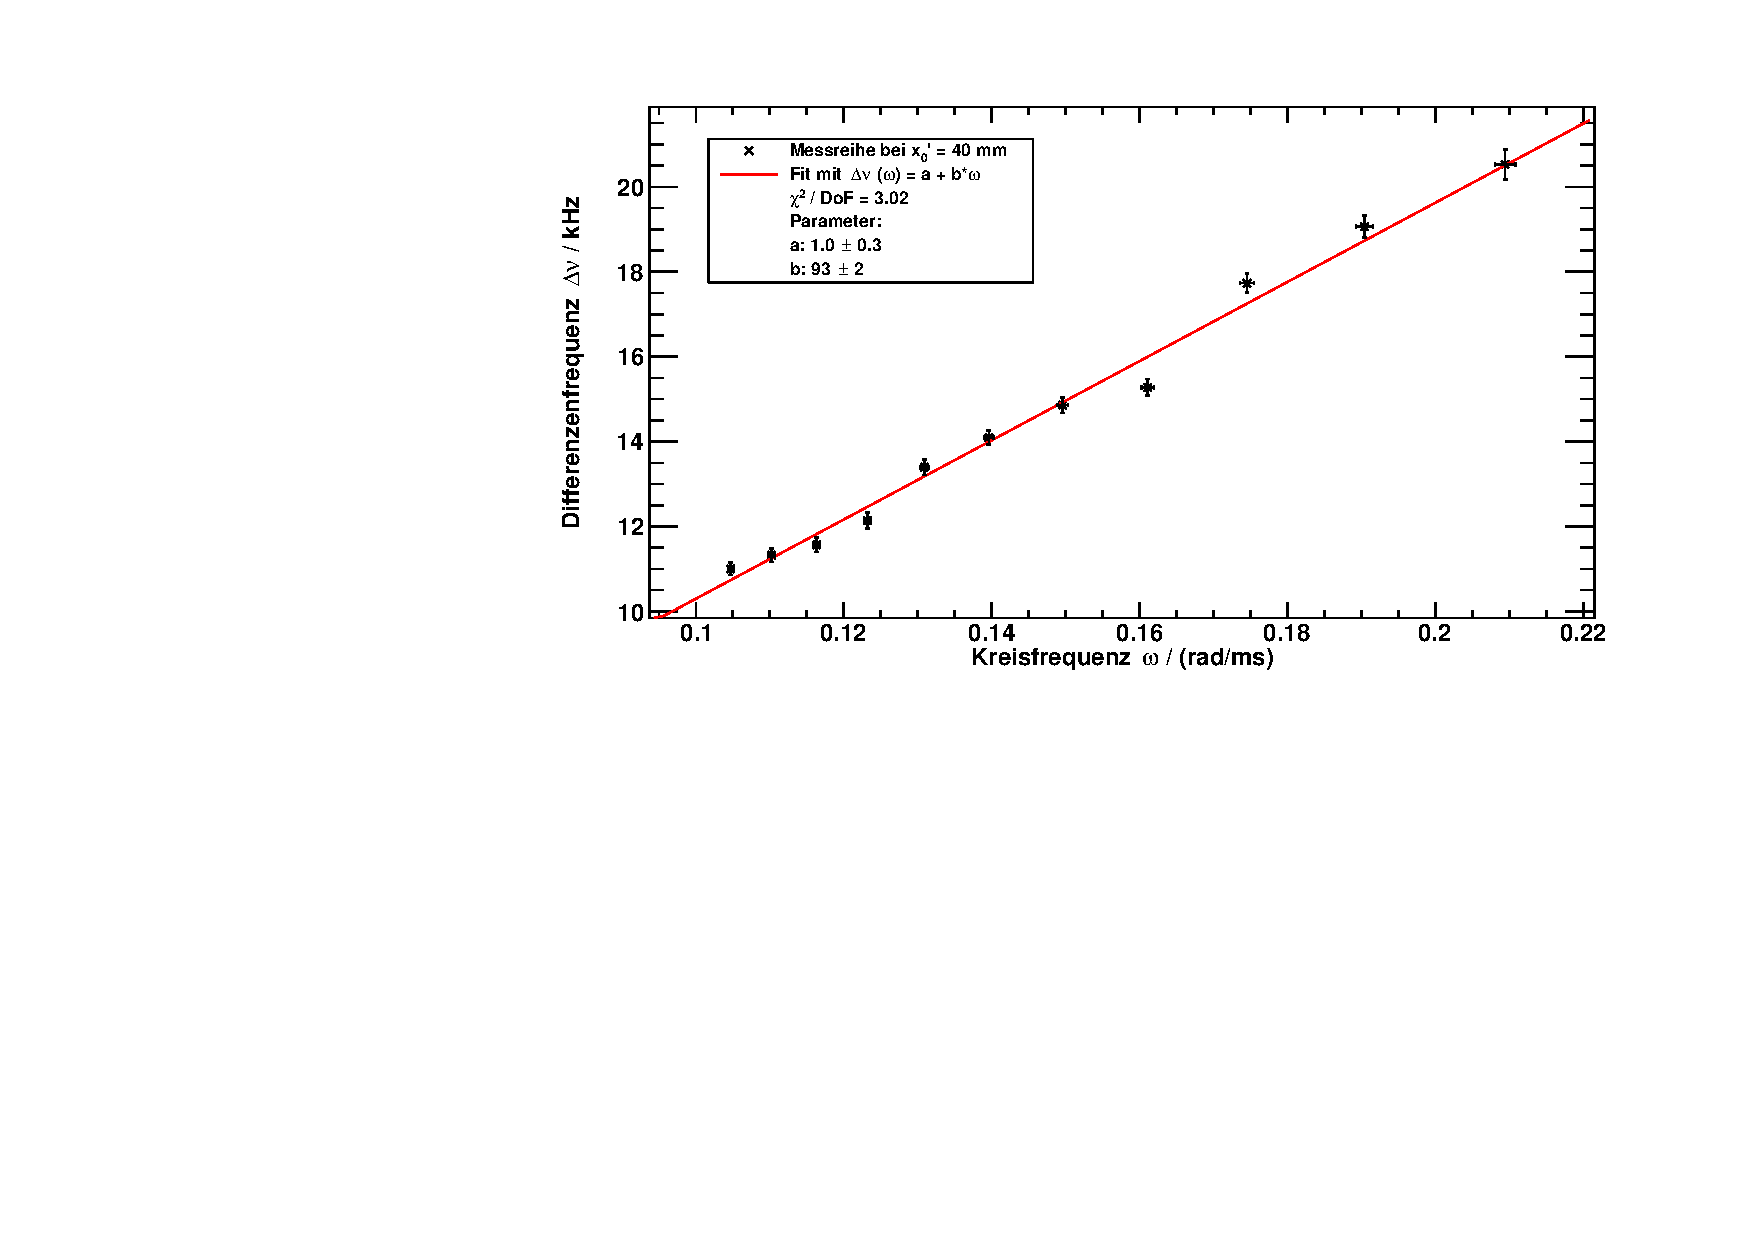
\includegraphics[width=\textwidth]{../img/fit_x0_40mm.pdf}
  \caption{Linearer Fit von $\Delta \nu$ bei $x_0' = 40$\,mm.}
  \label{img:fit:T:40mm}
\end{center}
\end{figure}

\begin{figure}[H]
\begin{center}
  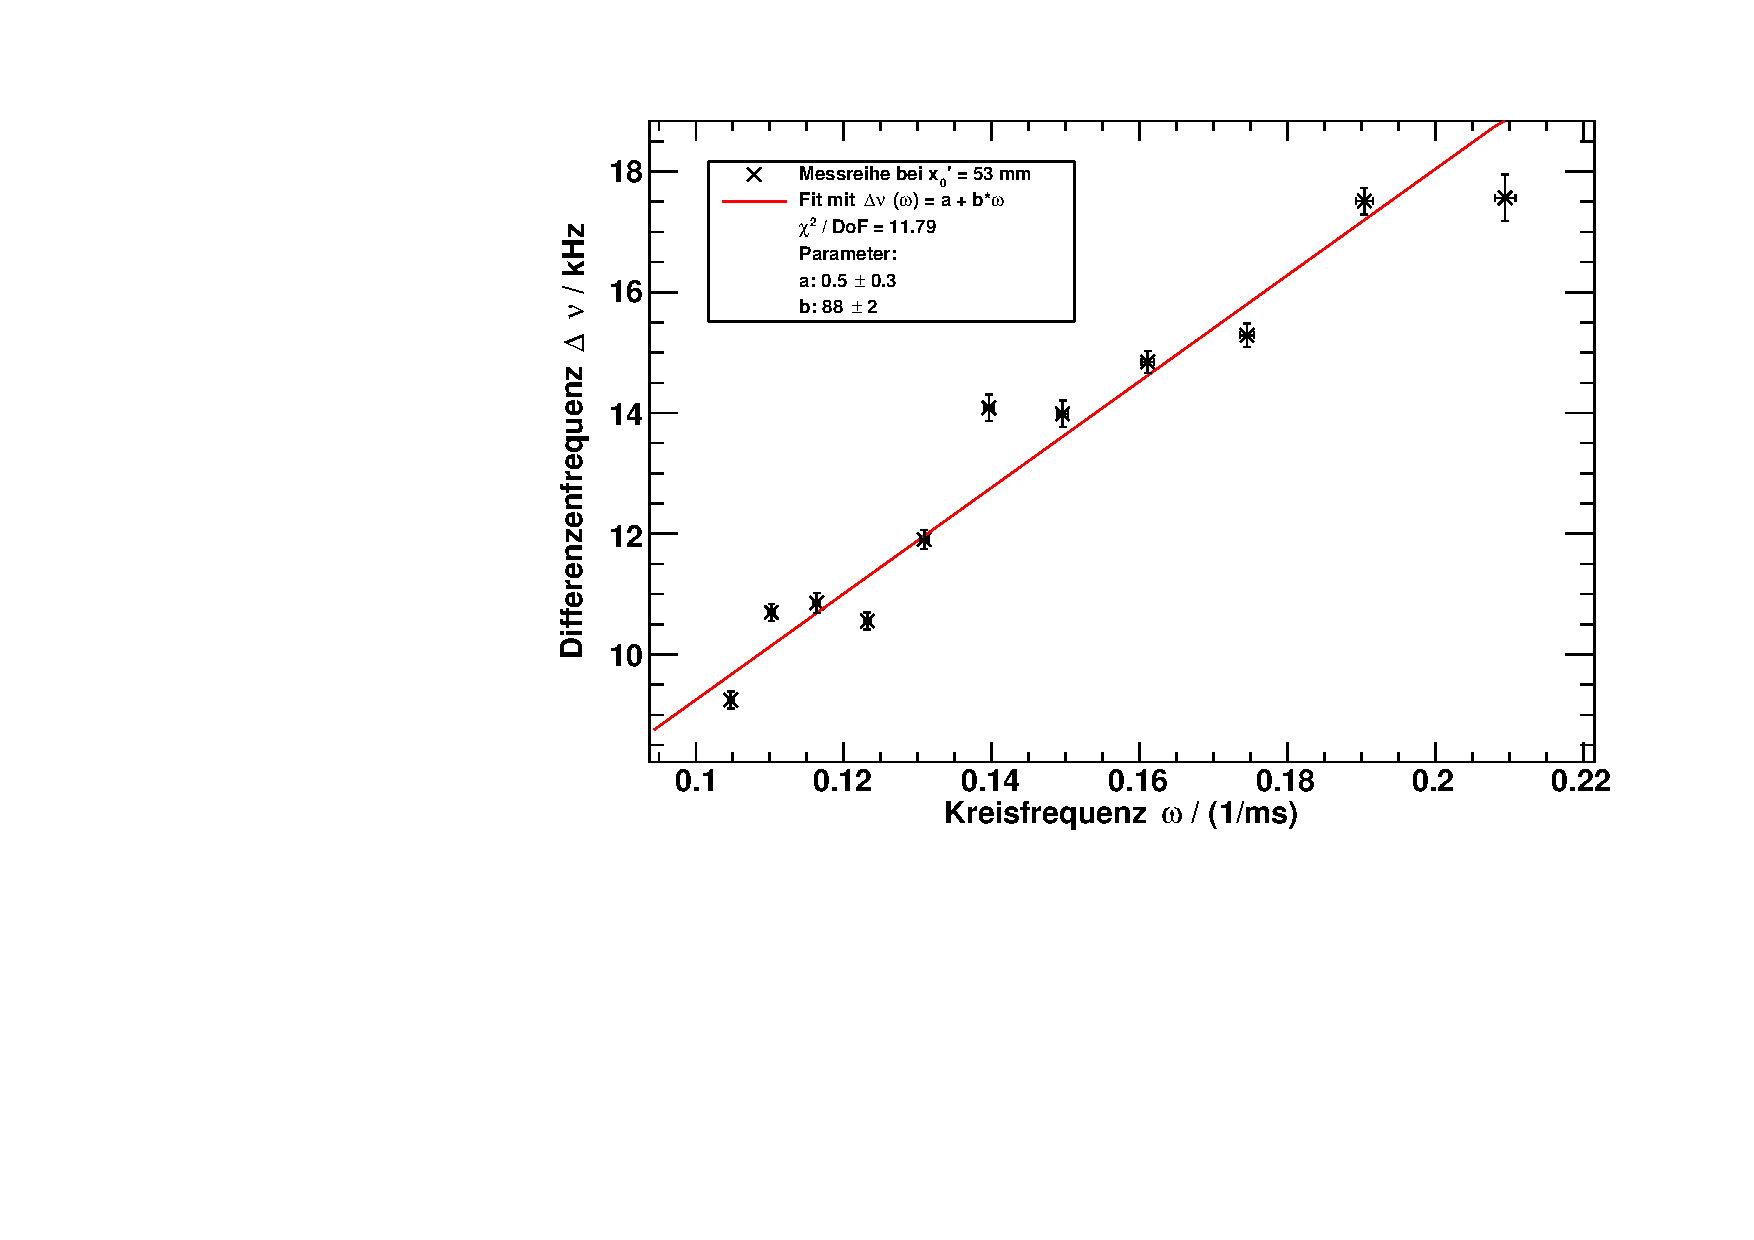
\includegraphics[width=\textwidth]{../img/fit_x0_53mm.pdf}
  \caption{Linearer Fit von $\Delta \nu$ bei $x_0' = 53$\,mm.}
  \label{img:fit:T:53mm}
\end{center}
\end{figure}

\begin{figure}[H]
\begin{center}
  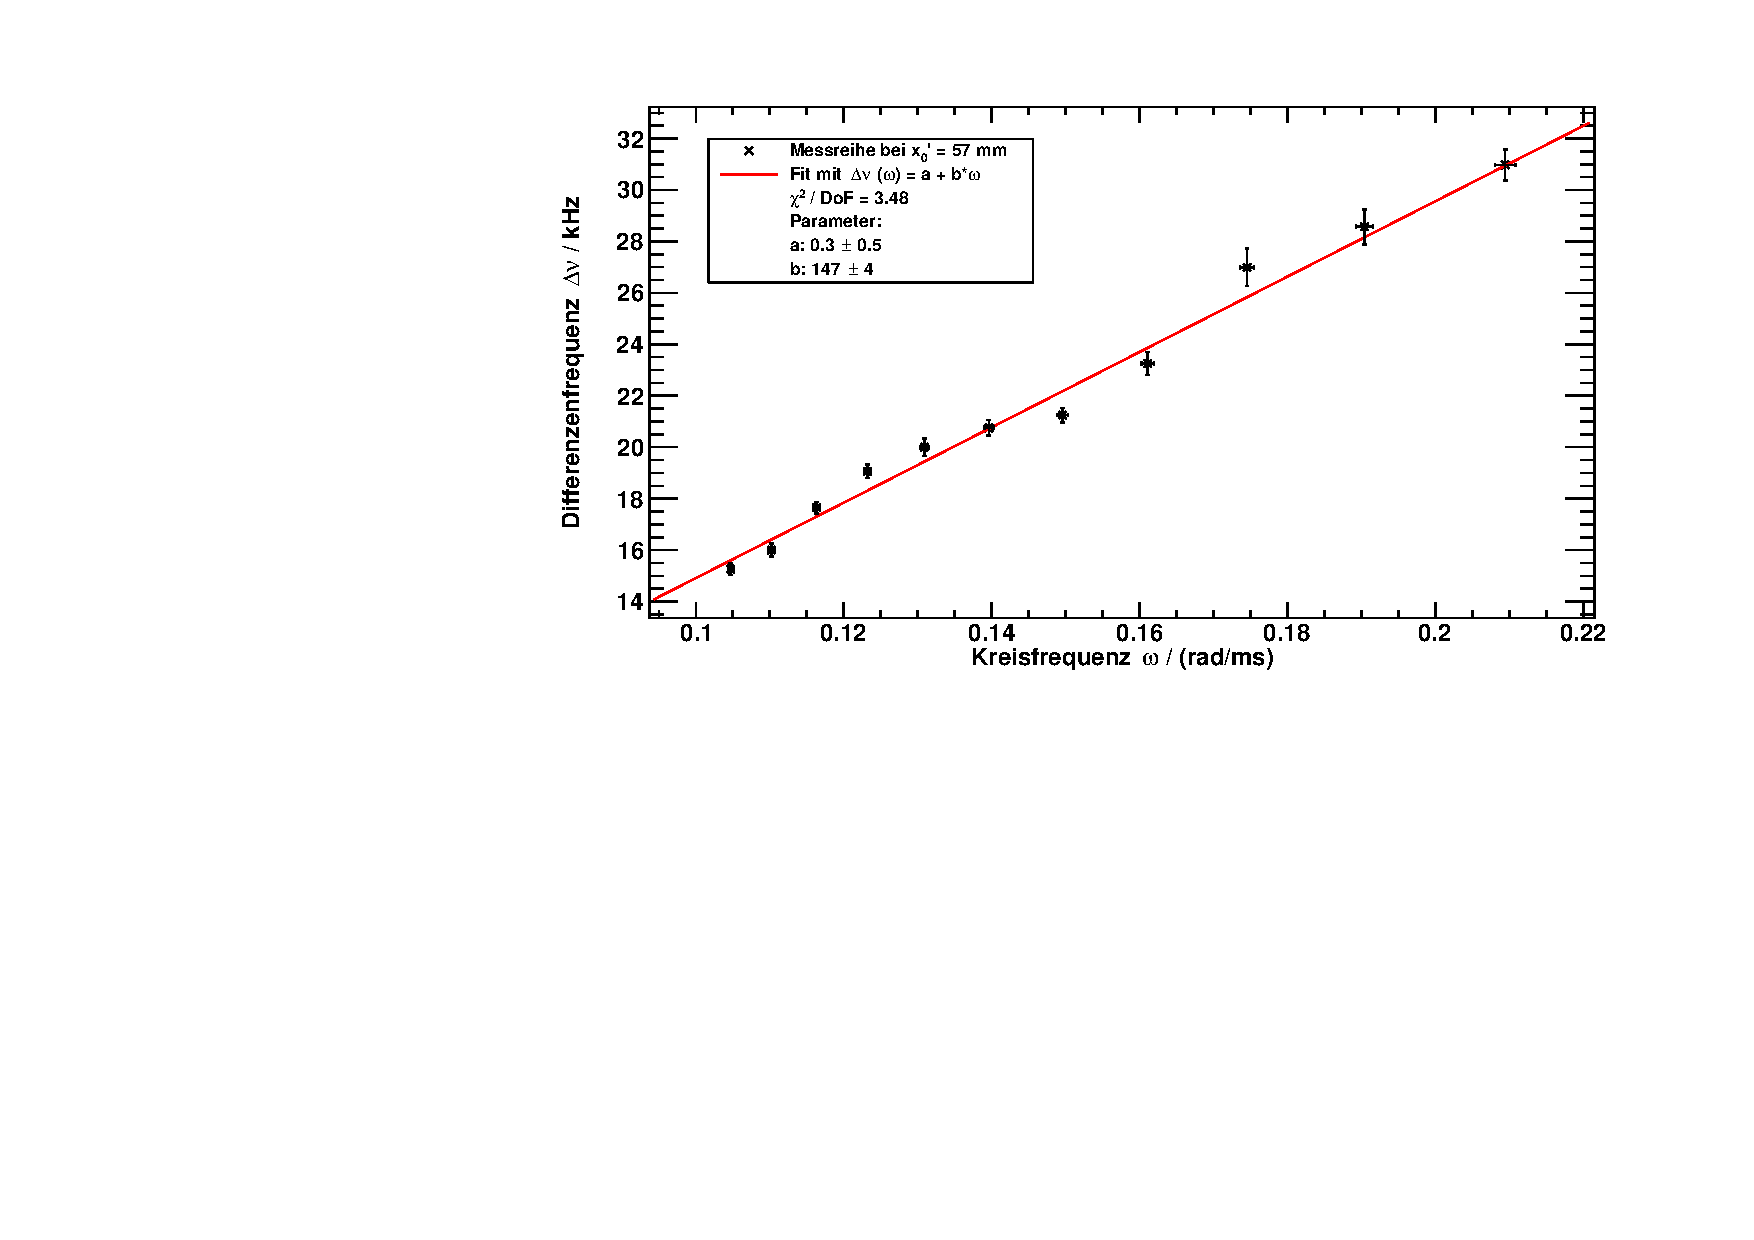
\includegraphics[width=\textwidth]{../img/fit_x0_57mm.pdf}
  \caption{Linearer Fit von $\Delta \nu$ bei $x_0' = 57$\,mm.}
  \label{img:fit:T:57mm}
\end{center}
\end{figure}

\begin{table}[H]
\caption{Fitergebnisse von $\Delta \nu(\omega)$ bei festen Auftrittpunkten $x_0'$.}
\begin{center}
\begin{tabular}{|c|c|c|c|c|}
  \hline
  $x_0'$ / mm & $a$ / kHz & $s_{a}$ / kHz & $b$ / (kHz $\cdot$ ms / rad) & $s_b$ / (kHz $\cdot$ ms / rad) \\ \hline
  36 & -0.6 & 0.5 & 164 & 4 \\ \hline
  40 & 1.0 & 0.3 & 93 & 2 \\ \hline
  53 & 0.5 & 0.3 & 88 & 2 \\ \hline
  57 & 0.3 & 0.5 & 147 & 4 \\ \hline
\end{tabular}
\end{center}
\label{tab:fit:T}
\end{table}


Die Offsets $a$ verschwinden alle innerhalb von maximal 4 Standardabweichungen. Aus den Steigungen $b$ lässt sich nun mit \autoref{eq:nu_omega} 
der Mitführungskoeffizient $\alpha$ bestimmen (alle Konstanten aus \autoref{sec:aufbau}):
\begin{equation}
  \alpha = \frac{\lambda \cdot L}{2 \cdot n \cdot d} \cdot \frac{b}{x_0}, \qquad
  s_\alpha = \alpha \cdot \sqrt{ \left( \frac{s_b}{b} \right)^2 + \left( \frac{s_{x_0}}{x_0} \right)^2 }
\end{equation}
Der Auftreffpunkt $x_0$ berechnet sich aus dem gemessenen Auftreffpunkt $s_0'$ (Fehler $s_{x_0'} = 0.05$\,mm) und dem 
Offset des Auftreffpunkts $x_m$, welcher oben (\autoref{eq:xm}) bestimmt wurde.
\begin{equation}
  x_0 = x_0' - x_m, \qquad s_{x_0} = \sqrt{s_{x_0'}^2 + s_{x_m}^2}
\end{equation}
Die verschiedenen Mitführungskoeffizienten sind in \autoref{tab:T:alpha} aufgelistet.
\begin{table}[H]
\caption{Mitf\"uhrungskoeffizienten bei festen Auftreffpunkten $x_0'$. }
\begin{center}
\begin{tabular}{|c|c|c|}
  \hline
  $T$ / ms & $\alpha$ & $s_{\alpha}$ \\ \hline
  36 & 0.554 & 0.014 \\ \hline
  40 & 0.498 & 0.012 \\ \hline
  53 & 0.529 & 0.013 \\ \hline
  57 & 0.532 & 0.016 \\ \hline
\end{tabular}
\end{center}
\label{tab:T:alpha}
\end{table}

Sie stimmen innerhalb von drei Standardabweichungen überein, deshalb kann wieder der gewichtete Mittelwert $\bar{\alpha}$ gebildet werden.
\begin{equation}
  \bar{\alpha} = 0.526 \pm 0.007
\end{equation}

\subsection{Vergleich der verschiedenen Mitführungskoeffizienten}
Der theoretsiche Mitführungskoeffizient $\alpha_{\text{theo}}$ lässt sich mit \autoref{eq:alpha:theo} mit dem Brechungsindex von Quarz $n=1.457$ 
und der Dispersion $\frac{\difd n}{\difd \lambda} = -300\,\text{cm}^{-1}$ bei der Wellenlänge $\lambda = 632.8$\,nm berechnen.
\begin{equation}
  \alpha_{\text{theo}} \approx 0.542
\end{equation}
Es werden zum Vergleich nochmal die berechneten Mitführungskoeffizienten bei variablen Periodendauern $\alpha_T$ und bei variablen Auftreffpunkten 
$\alpha_{x_0}$ aufgelistet.
\begin{equation}
\begin{split}
  \alpha_T = 0.526 \pm 0.007 \\
  \alpha_{x_0} = 0.536 \pm 0.002
\end{split}
\end{equation}
Sie stimmen innerhalb von zwei Standardabweichungen überein und der gewichtete Mittelwert lautet:
\begin{equation}
  \alpha_{\text{exp}} = 0.535 \pm 0.002
\end{equation}
Der theoretische Wert liegt innerhalb des $4$-$\sigma$-Intervalls dieses Wertes.